% Options for packages loaded elsewhere
% Options for packages loaded elsewhere
\PassOptionsToPackage{unicode}{hyperref}
\PassOptionsToPackage{hyphens}{url}
%
\documentclass[
  ignorenonframetext,
  aspectratio=169,
]{beamer}
\newif\ifbibliography
\usepackage{pgfpages}
\setbeamertemplate{caption}[numbered]
\setbeamertemplate{caption label separator}{: }
\setbeamercolor{caption name}{fg=normal text.fg}
\beamertemplatenavigationsymbolsempty
% remove section numbering
\setbeamertemplate{part page}{
  \centering
  \begin{beamercolorbox}[sep=16pt,center]{part title}
    \usebeamerfont{part title}\insertpart\par
  \end{beamercolorbox}
}
\setbeamertemplate{section page}{
  \centering
  \begin{beamercolorbox}[sep=12pt,center]{section title}
    \usebeamerfont{section title}\insertsection\par
  \end{beamercolorbox}
}
\setbeamertemplate{subsection page}{
  \centering
  \begin{beamercolorbox}[sep=8pt,center]{subsection title}
    \usebeamerfont{subsection title}\insertsubsection\par
  \end{beamercolorbox}
}
% Prevent slide breaks in the middle of a paragraph
\widowpenalties 1 10000
\raggedbottom
\usepackage{iftex}
\ifPDFTeX
  \usepackage[T1]{fontenc}
  \usepackage[utf8]{inputenc}
  \usepackage{textcomp} % provide euro and other symbols
\else % if luatex or xetex
  \usepackage{unicode-math} % this also loads fontspec
  \defaultfontfeatures{Scale=MatchLowercase}
  \defaultfontfeatures[\rmfamily]{Ligatures=TeX,Scale=1}
\fi
\usepackage{lmodern}

\ifPDFTeX\else
  % xetex/luatex font selection
\fi
% Use upquote if available, for straight quotes in verbatim environments
\IfFileExists{upquote.sty}{\usepackage{upquote}}{}
\IfFileExists{microtype.sty}{% use microtype if available
  \usepackage[]{microtype}
  \UseMicrotypeSet[protrusion]{basicmath} % disable protrusion for tt fonts
}{}
\makeatletter
\@ifundefined{KOMAClassName}{% if non-KOMA class
  \IfFileExists{parskip.sty}{%
    \usepackage{parskip}
  }{% else
    \setlength{\parindent}{0pt}
    \setlength{\parskip}{6pt plus 2pt minus 1pt}}
}{% if KOMA class
  \KOMAoptions{parskip=half}}
\makeatother


\usepackage{longtable,booktabs,array}
\usepackage{calc} % for calculating minipage widths
\usepackage{caption}
% Make caption package work with longtable
\makeatletter
\def\fnum@table{\tablename~\thetable}
\makeatother
\usepackage{graphicx}
\makeatletter
\newsavebox\pandoc@box
\newcommand*\pandocbounded[1]{% scales image to fit in text height/width
  \sbox\pandoc@box{#1}%
  \Gscale@div\@tempa{\textheight}{\dimexpr\ht\pandoc@box+\dp\pandoc@box\relax}%
  \Gscale@div\@tempb{\linewidth}{\wd\pandoc@box}%
  \ifdim\@tempb\p@<\@tempa\p@\let\@tempa\@tempb\fi% select the smaller of both
  \ifdim\@tempa\p@<\p@\scalebox{\@tempa}{\usebox\pandoc@box}%
  \else\usebox{\pandoc@box}%
  \fi%
}
% Set default figure placement to htbp
\def\fps@figure{htbp}
\makeatother





\setlength{\emergencystretch}{3em} % prevent overfull lines

\providecommand{\tightlist}{%
  \setlength{\itemsep}{0pt}\setlength{\parskip}{0pt}}



 


% nf-macros.tex — visual building blocks for "Metodi Statistici per la Neuropsicologia Forense"
% Adapted from the Time Management deck (tm-macros.tex); loads unipdwarsawstyle.sty first.

% ---------------------------------------------------------
% FONTS, ICONS, LIBRARIES
% ---------------------------------------------------------
\usepackage{unipdwarsawstyle}
\usepackage[sfdefault]{FiraSans}
\usepackage{fontawesome5}
\usetikzlibrary{arrows.meta,positioning,calc,fit,backgrounds,shapes.geometric}

% ---------------------------------------------------------
% IMAGE HEIGHT CAP — 16:9 frames are shorter than the old 4:3 ones, so images sized
% by width can run off the bottom. Every \includegraphics taller than \nfmaxheight
% is scaled down (aspect ratio kept); unsized markdown images use the same limit.
% ---------------------------------------------------------
\newlength{\nfmaxheight}
\AtBeginDocument{\setlength{\nfmaxheight}{0.74\textheight}}
\makeatletter
\newsavebox\nf@imgbox
\let\nf@includegraphics\includegraphics
\renewcommand*\includegraphics[2][]{%
  \sbox\nf@imgbox{\nf@includegraphics[#1]{#2}}%
  \ifdim\dimexpr\ht\nf@imgbox+\dp\nf@imgbox\relax>\nfmaxheight
    \resizebox{!}{\nfmaxheight}{\usebox\nf@imgbox}%
  \else\usebox\nf@imgbox\fi}
% unsized markdown images: fit within \linewidth and \nfmaxheight
\renewcommand*\pandocbounded[1]{%
  \sbox\nf@imgbox{#1}%
  \Gscale@div\@tempa{\nfmaxheight}{\dimexpr\ht\nf@imgbox+\dp\nf@imgbox\relax}%
  \Gscale@div\@tempb{\linewidth}{\wd\nf@imgbox}%
  \ifdim\@tempb\p@<\@tempa\p@\let\@tempa\@tempb\fi
  \ifdim\@tempa\p@<\p@\scalebox{\@tempa}{\usebox\nf@imgbox}\else\usebox\nf@imgbox\fi}
\makeatother

% ---------------------------------------------------------
% PALETTE — structure is UniPD crimson/gold (from the style file)
% ---------------------------------------------------------
\definecolor{nfInk}{HTML}{243447}      % dark text
\definecolor{nfPoll}{HTML}{5B3F9E}     % Wooclap
\definecolor{nfPadlet}{HTML}{B8860B}   % Padlet
\definecolor{nfGrey}{HTML}{8A94A0}

% ---------------------------------------------------------
% GLOBAL LOOK
% ---------------------------------------------------------
\hyphenpenalty=10000 \exhyphenpenalty=10000
\setbeamertemplate{headline}{}
\setbeamercolor{background canvas}{bg=white}
\setbeamercolor{normal text}{fg=nfInk}
\setbeamerfont{frametitle}{size=\large,series=\bfseries}
\setbeamertemplate{footline}{%
  \hfill{\color{nfGrey}\tiny\insertframenumber}\hspace*{4mm}\vspace*{2mm}}
\setbeamertemplate{itemize item}{\color{unipdCrimson}\raisebox{0.15ex}{\scriptsize\faCircle}}

% ---------------------------------------------------------
% ICON ROW — icon in a crimson disc + text
%   \iconrow{\faVideo}{Text}
% ---------------------------------------------------------
\newcommand{\iconrow}[2]{%
  \par\noindent
  \begin{minipage}[c]{0.9cm}\centering
    \tikz\node[circle, fill=unipdCrimson, text=white, minimum size=7mm, inner sep=0pt]{\small #1};
  \end{minipage}%
  \begin{minipage}[c]{\dimexpr\linewidth-0.9cm\relax}\small #2\end{minipage}\par\vspace{5pt}}

% ---------------------------------------------------------
% ACTIVITIES — real QR code and join code
% ---------------------------------------------------------
\newcommand{\timer}[1]{%
  \tikz[baseline=(t.base)]\node[fill=unipdCrimson, text=white, rounded corners=6pt,
    font=\scriptsize\bfseries, inner sep=3pt] (t) {\faIcon{stopwatch}\ #1};}

%   \qrbox{colour}{Figures/qr.png}{code or empty}
\newcommand{\qrbox}[3]{%
  \begin{tikzpicture}
    \node[draw=#1, line width=1.2pt, rounded corners=5pt, inner sep=5pt, fill=white] (q)
      {\includegraphics[width=3.4cm]{#2}};
    \if\relax\detokenize{#3}\relax\else
      \node[below=3pt of q, font=\small\bfseries\color{#1}] {codice: #3};
    \fi
  \end{tikzpicture}}

%   \wooclapslot{tipo}{domanda}{istruzioni}{minuti o vuoto}{Figures/qr.png}{codice}
\newcommand{\wooclapslot}[6]{%
  \begin{columns}[c]
    \begin{column}{0.56\textwidth}
      {\color{nfPoll}\small\faPoll\ \textbf{WOOCLAP}\,·\,#1}%
      \if\relax\detokenize{#4}\relax\else\hfill\timer{#4}\fi\par\vspace{8pt}
      {\LARGE\bfseries\color{nfInk}#2\par}\vspace{10pt}
      {\small\color{nfInk}#3\par}
    \end{column}
    \begin{column}{0.40\textwidth}\centering\qrbox{nfPoll}{#5}{#6}\end{column}
  \end{columns}}

%   \padletslot{tipo}{domanda}{istruzioni}{minuti o vuoto}{Figures/qr.png}
\newcommand{\padletslot}[5]{%
  \begin{columns}[c]
    \begin{column}{0.56\textwidth}
      {\color{nfPadlet}\small\faStickyNote\ \textbf{PADLET}\,·\,#1}%
      \if\relax\detokenize{#4}\relax\else\hfill\timer{#4}\fi\par\vspace{8pt}
      {\LARGE\bfseries\color{nfInk}#2\par}\vspace{10pt}
      {\small\color{nfInk}#3\par}
    \end{column}
    \begin{column}{0.40\textwidth}\centering\qrbox{nfPadlet}{#5}{}\end{column}
  \end{columns}}

% ---------------------------------------------------------
% TITLE SLIDE — use on a  ## {.plain}  frame:   \nftitleslide{2 · Cornice teorica}
% ---------------------------------------------------------
\newcommand{\nftitleslide}[1]{%
  \begin{tikzpicture}[remember picture, overlay]
    \fill[unipdCrimson] (current page.north west) rectangle ([xshift=0.58\paperwidth]current page.south west);
    \fill[unipdGold] ([xshift=0.58\paperwidth]current page.north west) rectangle ([xshift=0.585\paperwidth]current page.south west);
  \end{tikzpicture}%
  \begin{columns}[c]
    \begin{column}{0.55\textwidth}
      \color{white}
      {\small\color{unipdGold}\MakeUppercase{#1}\par}\vspace{6pt}
      {\fontsize{22}{27}\selectfont\bfseries Metodi Statistici per la Neuropsicologia Forense\par}\vspace{22pt}
      {\small\bfseries Giorgio Arcara\par}
      {\scriptsize Università di Padova\\ IRCCS San Camillo, Venezia\par}
    \end{column}
    \begin{column}{0.40\textwidth}\centering
      
\includegraphics[width=0.85\linewidth]{Figures/LogoSanCamilloIRCCS_Unipd_alpha.png}\par\vspace{14pt}
      
\includegraphics[height=0.55cm]{Figures/CC_license_3_0.png}
    \end{column}
  \end{columns}}

% ---------------------------------------------------------
% SECTION DIVIDER — built automatically from each "# Section" heading
% (YAML: section-titles: false, so Quarto does not add its own)
% ---------------------------------------------------------
\AtBeginSection{%
  \begin{frame}[plain]
    \begin{tikzpicture}[remember picture, overlay]
      \fill[unipdCrimson] (current page.north west) rectangle ([xshift=3mm]current page.south west);
      \fill[unipdGold] ([xshift=3mm]current page.north west) rectangle ([xshift=3.6mm]current page.south west);
      \node[anchor=north west, font=\scriptsize\color{nfGrey}, inner sep=0pt]
        at ([xshift=8mm,yshift=-5mm]current page.north west)
        {METODI STATISTICI PER LA NEUROPSICOLOGIA FORENSE};
    \end{tikzpicture}
    \vfill
    \begin{center}
      {\fontsize{26}{32}\selectfont\bfseries\color{unipdCrimson}\insertsectionhead\par}
    \end{center}
    \vfill
  \end{frame}}

% ---------------------------------------------------------
% TAKEAWAY strip at the bottom of the slide
% ---------------------------------------------------------
\newcommand{\takeaway}[1]{%
  \begin{tikzpicture}[remember picture, overlay]
    \node[anchor=south west, fill=unipdCream!70, text=nfInk, font=\scriptsize,
          inner xsep=6pt, inner ysep=3pt, rounded corners=2pt, text width=0.84\paperwidth]
      at ([xshift=5mm,yshift=4mm]current page.south west)
      {\textcolor{unipdCrimson}{\faKey}\ \textbf{In sintesi:} #1};
  \end{tikzpicture}}
\makeatletter
\@ifpackageloaded{caption}{}{\usepackage{caption}}
\AtBeginDocument{%
\ifdefined\contentsname
  \renewcommand*\contentsname{Table of contents}
\else
  \newcommand\contentsname{Table of contents}
\fi
\ifdefined\listfigurename
  \renewcommand*\listfigurename{List of Figures}
\else
  \newcommand\listfigurename{List of Figures}
\fi
\ifdefined\listtablename
  \renewcommand*\listtablename{List of Tables}
\else
  \newcommand\listtablename{List of Tables}
\fi
\ifdefined\figurename
  \renewcommand*\figurename{Figure}
\else
  \newcommand\figurename{Figure}
\fi
\ifdefined\tablename
  \renewcommand*\tablename{Table}
\else
  \newcommand\tablename{Table}
\fi
}
\@ifpackageloaded{float}{}{\usepackage{float}}
\floatstyle{ruled}
\@ifundefined{c@chapter}{\newfloat{codelisting}{h}{lop}}{\newfloat{codelisting}{h}{lop}[chapter]}
\floatname{codelisting}{Listing}
\newcommand*\listoflistings{\listof{codelisting}{List of Listings}}
\makeatother
\makeatletter
\makeatother
\makeatletter
\@ifpackageloaded{caption}{}{\usepackage{caption}}
\@ifpackageloaded{subcaption}{}{\usepackage{subcaption}}
\makeatother

\usepackage{bookmark}
\IfFileExists{xurl.sty}{\usepackage{xurl}}{} % add URL line breaks if available
\urlstyle{same}
\hypersetup{
  pdfauthor={Giorgio Arcara},
  hidelinks,
  pdfcreator={LaTeX via pandoc}}


\author{Giorgio Arcara}
\date{}

\begin{document}


\begin{frame}[plain]{}
\phantomsection\label{section}
\nftitleslide{8a · La scelta dei test per la propria cassetta degli attrezzi}
\end{frame}

\section{La scelta dei test per la propria cassetta degli
attrezzi}\label{la-scelta-dei-test-per-la-propria-cassetta-degli-attrezzi}

\begin{frame}{La scelta dei test}
\phantomsection\label{la-scelta-dei-test}
Due momenti di scelta dei test:

\begin{enumerate}[<+->]
[1)]
\item
  \textbf{Scelta dei test da inserire nella propria ``cassetta degli
  attrezzi''}
\item
  Scelta dei test da utilizzare con uno specifico individuo per uno
  specifico scopo.
\end{enumerate}
\end{frame}

\begin{frame}{\small La scelta dei test da inserire nella propria
«cassetta degli attrezzi»}
\phantomsection\label{la-scelta-dei-test-da-inserire-nella-propria-cassetta-degli-attrezzi}
\emph{Regole generali da seguire}

Test che abbiano caratteristiche psicometriche soddisfacenti (validità,
affidabilità, dati normativi adeguati,
\underline{visti nei blocchi precedenti})

Dipende molto da fattori pratici: il tipo di realtà clinica o forense
nella quale si utilizzano i test influenza quali sono i test da
utilizzare potenzialmente.
\end{frame}

\begin{frame}{\small La scelta dei test da inserire nella propria
«cassetta degli attrezzi»}
\phantomsection\label{la-scelta-dei-test-da-inserire-nella-propria-cassetta-degli-attrezzi-1}
\emph{Come selezionare i test?}

\underline{Possibili fonti:}

\textbf{Kit del Neuropsicologo}: un libro prodotto dalla Società
Italiana di Neuropsicologia (per i Soci) che contiene riferimenti a
quasi tutti i test disponibili in Italiano (non è però aggiornatissimo
ed è difficile da trovare).

\textbf{Libro ``L'esame neuropsicologico dell'Adulto''} (a cura di
Bianchi A.): contiene un capitolo che include una lista piuttosto ampia
di test neuropsicologici adattati in Italiano.

\textbf{Corso: Valutazione delle funzioni cognitive in ambito forense}:
Presso il vostro corso di laurea.
\end{frame}

\begin{frame}{\small La scelta dei test da inserire nella propria
«cassetta degli attrezzi»}
\phantomsection\label{la-scelta-dei-test-da-inserire-nella-propria-cassetta-degli-attrezzi-2}
\emph{Come selezionare i test?}

\underline{Possibili fonti:}

\textbf{Case editrici di test (Organizzazioni Speciali, Erickson)}: sono
test a pagamento che garantiscono un certo standard di qualità.
\end{frame}

\begin{frame}{\small La scelta dei test da inserire nella propria
«cassetta degli attrezzi»}
\phantomsection\label{la-scelta-dei-test-da-inserire-nella-propria-cassetta-degli-attrezzi-3}
\begin{center}
  \textbf{METODI CHE SUGGERISCO}
\end{center}

\textbf{Docenti universitari, futuri colleghi ed esperti di un certo
settore/patologia}: è il modo migliore (se trovate qualcuno disponibile
a condividere le informazioni).

\textbf{Articoli scientifici/consensus specifici per patologia}: Cercate
(es. su scholar o pubmed, se ci sono linee guida o criteri e cercate se
i test sono validati/standardizzati in Italiano).

\textbf{Attese da mondo forense}: è possibile che nel mondo forense ci
si attenda determinati test. Per quanto il messaggio di usare i test
migliori possibili permane, bisogna anche tenere conto che ci si
potrebbe aspettare certi test (es. WAIS per Q.I.) e potrebbe non essere
strategico selezionarne alcuni che la/il giudice non capisce/a cui non è
familiare.
\end{frame}

\begin{frame}{\small La scelta dei test da inserire nella propria
«cassetta degli attrezzi»}
\phantomsection\label{la-scelta-dei-test-da-inserire-nella-propria-cassetta-degli-attrezzi-4}
\textbf{Articoli scientifici/consensus}

Ricordate che avere l'articolo scientifico spesso non basta. Serve anche
avere il manuale di istruzioni e di somministrazione (e attribuzione dei
punteggi) e i materiali del test, eventuali tabelle dei dati normativi

Utilizzate con cautela test di cui non avete referenze ufficiali
(possono avere modifiche ``custom'', che alterano il test)

\emph{Contattate gli autori del test (la mail è presente nell'articolo)
e chiedete se è disponibile.}
\end{frame}

\begin{frame}{La scelta dei test da inserire nella propria «cassetta
degli attrezzi»}
\phantomsection\label{la-scelta-dei-test-da-inserire-nella-propria-cassetta-degli-attrezzi-5}
\emph{Cosa evitare nella selezione dei test?}

\begin{itemize}[<*>] 
  \item Evitare test troppo datati (se i dati normativi sono troppo vecchi potrebbero non essere utilizzabili) – \emph{come visto nel blocco sui dati normativi}.
  \item Evitare test “fatti in casa”: un test passato da un collega senza dati normativi (magari tradotti da un test in inglese) può essere accattivante (e talvolta utile) ma è limitato nelle informazioni che può fornire – \emph{come visto nei blocchi su validità, affidabilità e dati normativi}.
  \item Evitare test che sono semplici traduzioni da test stranieri, non "adattati" all'italiano tramite opportune prove di validità, affidabilità e dati normativi.
\end{itemize}
\end{frame}

\begin{frame}{I criteri per cui scegliere i test per valutazioni in
ambito forense}
\phantomsection\label{i-criteri-per-cui-scegliere-i-test-per-valutazioni-in-ambito-forense}
\begin{columns}
\column{0.7\textwidth}

\textbf{1) Test adeguati alle potenziali domande delle valutazioni che dovrete fare}

\column{0.3\textwidth}

\begin{figure}
    
\includegraphics[scale=0.04]{Figures/triangle.png}
\end{figure}

\end{columns}
\pause
\vfill

\begin{columns}
\column{1\textwidth}

\textbf{2) Test con buone capacità psicometriche}
\begin{itemize}[<*>] 
  \item Test con buona validità
  \item Test con buona affidabilità
  \item Test con buone proprietà di altro tipo (es. Valori di cambiamento)
  \item Test con dati normativi adeguati.
\end{itemize}

\column{0\textwidth}
\end{columns}

\vfill

In generale non dimenticate il razionale: i test ci forniscono informazioni e parte di queste informazioni derivano dalle caratteristiche dei test.
\end{frame}

\begin{frame}{Scelta dei test}
\phantomsection\label{scelta-dei-test}
\pandocbounded{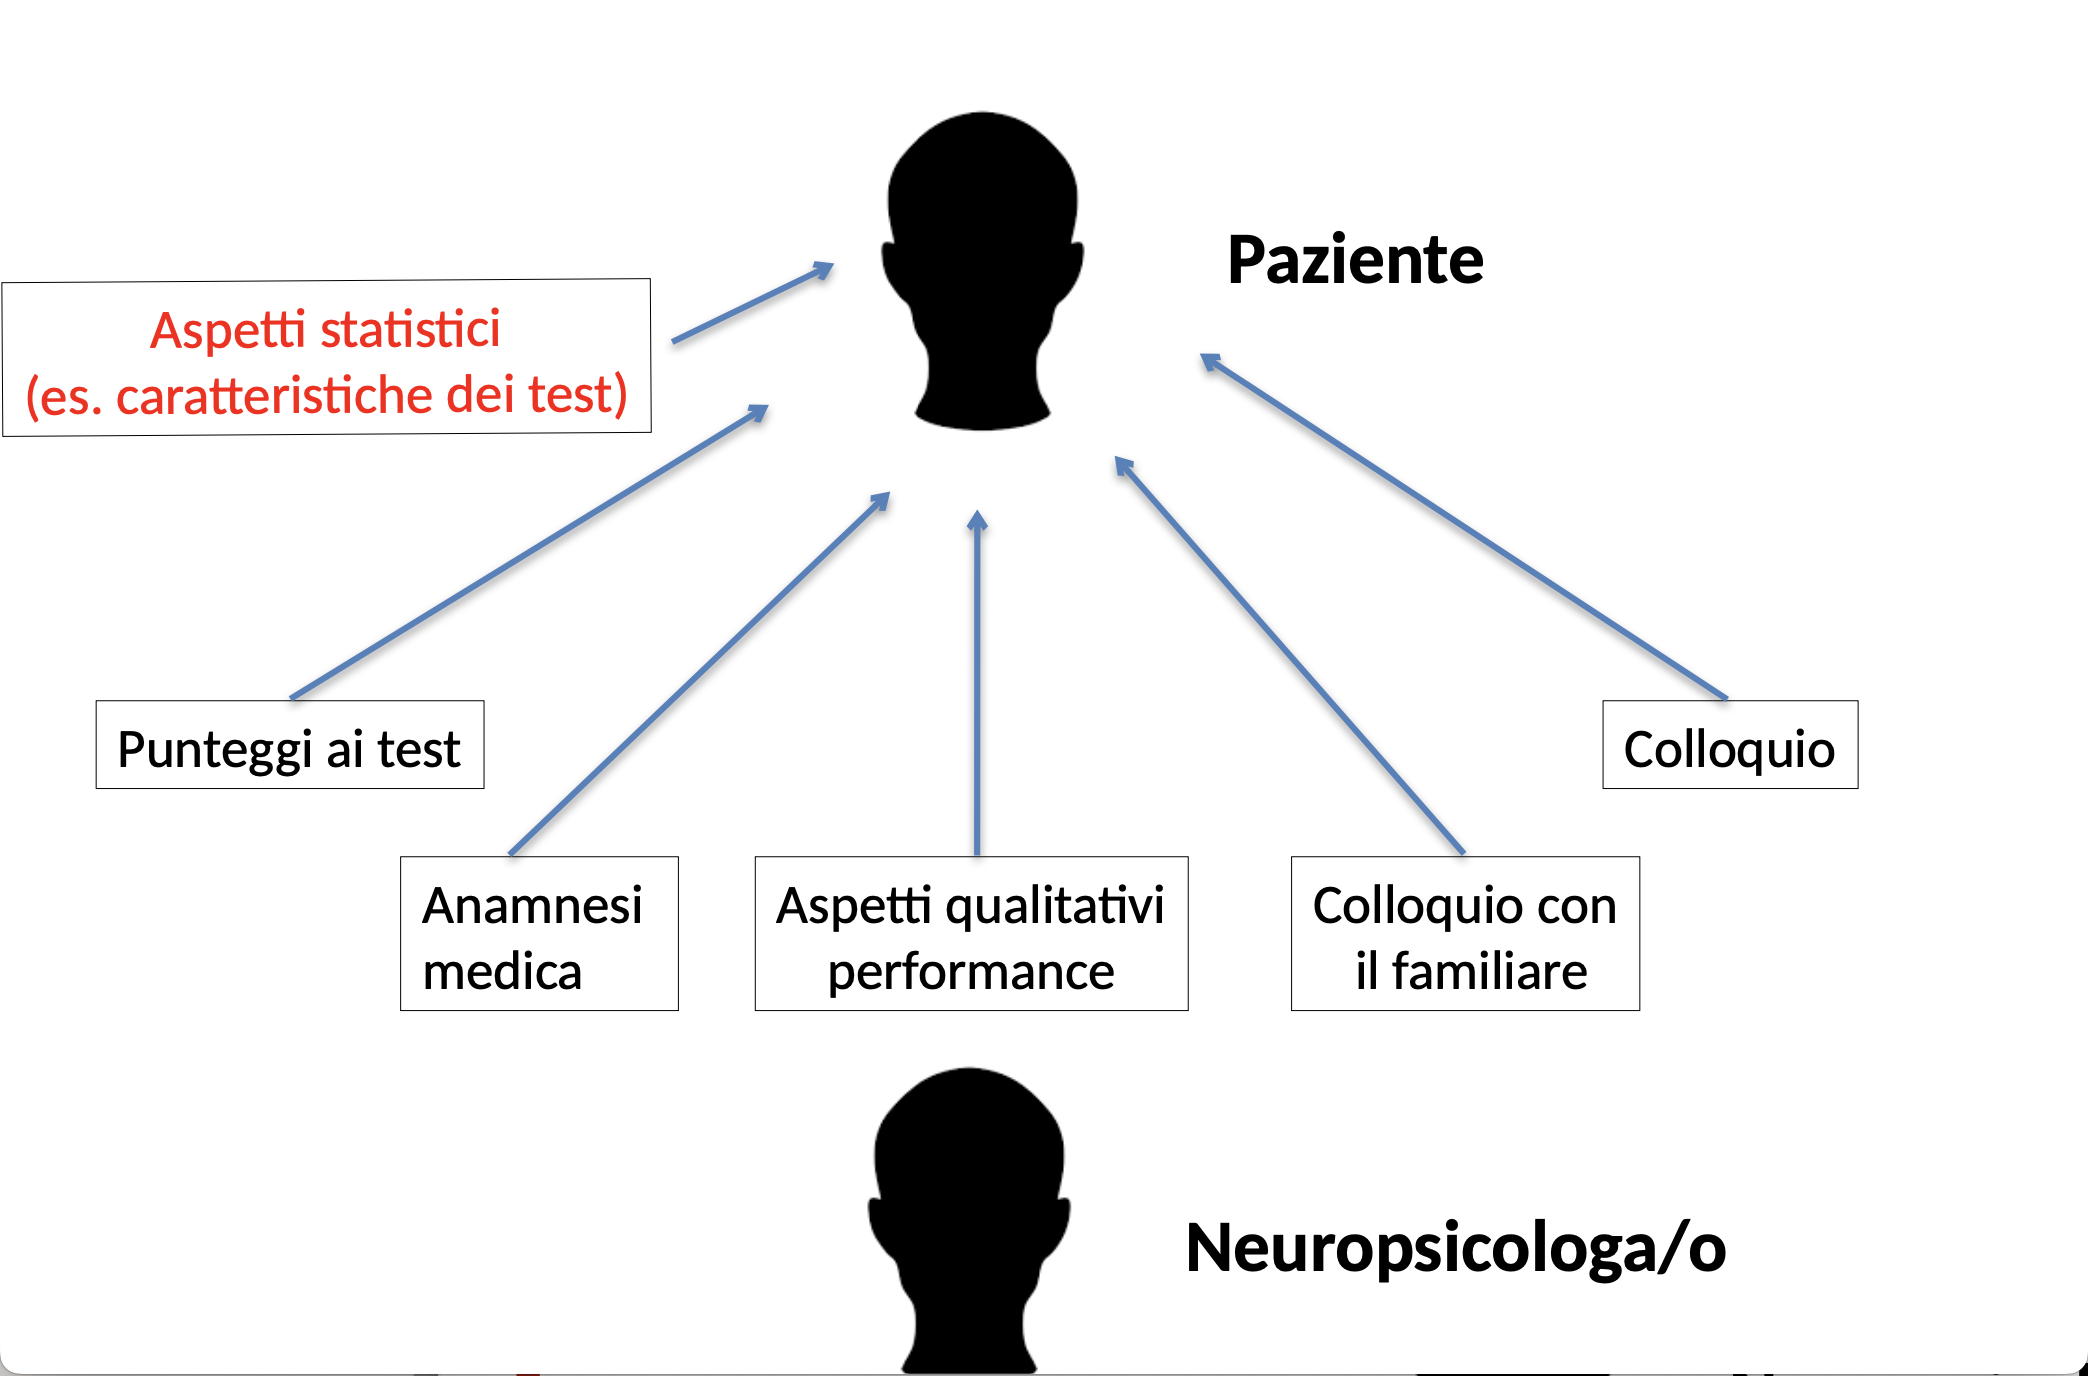
\includegraphics[keepaspectratio]{Figures/Active_collection.png}}
\end{frame}




\end{document}
